\documentclass[12pt,fleqn]{article}\usepackage{../../common}
\begin{document}
Ders 28

Önceki derste bir yüzey içinden olan akış hesabını gördük. Bu bir çift
entegraldi,

$$
\int \int_S \vec{F} \cdot \hat{n} \ud S
$$

ki $\hat{n}$ yüzeye olan birim normaldi, $\ud S$ ise yüzeydeki alan öğesi.
Gördük ki farklı yüzeyler için farklı $\hat{n}$ ve farklı alan öğe formülü
$\ud S$ olabiliyordu. Bulmamız gereken yüzeyin ufak bir parçası için
$\hat{n} \ud S$'in ne olacağını bulmak.

Diyelim ki yüzeyin $xy$ düzlemine olan yansımasındaki / ``gölgesindeki'' ufak
bir dikdörtgeni alıyoruz, ki bu dikdörtgenin kenarları $\Delta x$ ve $\Delta y$,
ve onun yüzey $S$'deki karşılığına bakıyoruz.

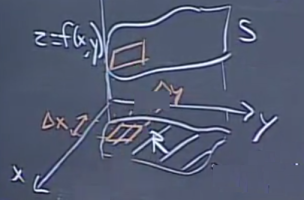
\includegraphics[width=20em]{calc_multi_28_01.png}












[devam edecek]

\end{document}
